Switched actuators are difficult to handle because of some characteristic constraints of their nature. 
But they are efficient in numerous engineering applications, being applied, for example, in attitude control systems for space vehicles. 
Thus, knowing how to use this type of actuator is important and necessary. 
The main problem to be solved in this thesis is the design of a controller that guarantees the robustness of a system with switched actuators subjected to time constraints 
that limit the response window of their commands.
In this approach, a limit cycle target trajectory search is performed and then the error of the states compared to the target trajectory is calculated. Then a predictive control technique 
is applied to correct the error and get the system to the cyclic target trajectory


% teste de escrita
% 84+ 9+ 84+ 9+ 84+ 9=279
%
%84+ 9+ 84+ 9+ 84+ 9=279
%
%
\begin{figure}[h!]
    \centering
    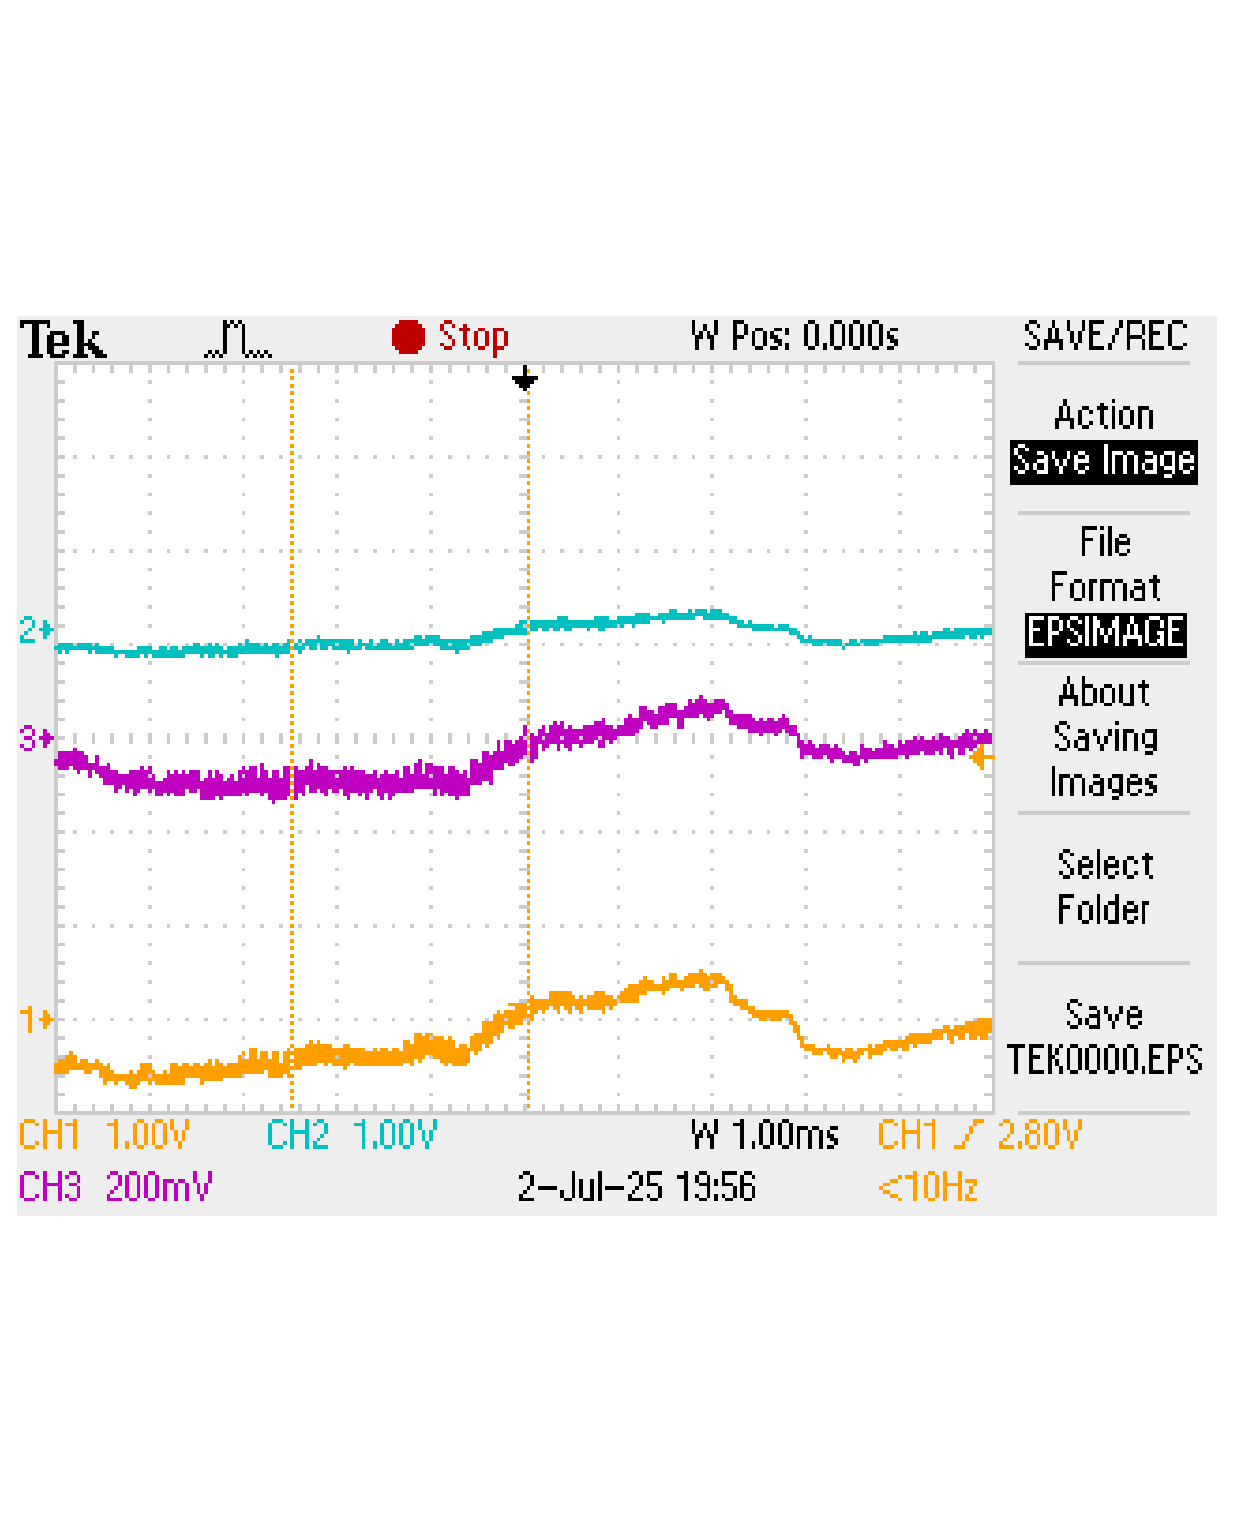
\includegraphics[]{figuras/TEK0000.EPS}
    \caption{figura teste}
    \label{asdfasdf}
\end{figure}

% \begin{figure}[h]
%     \centering
%     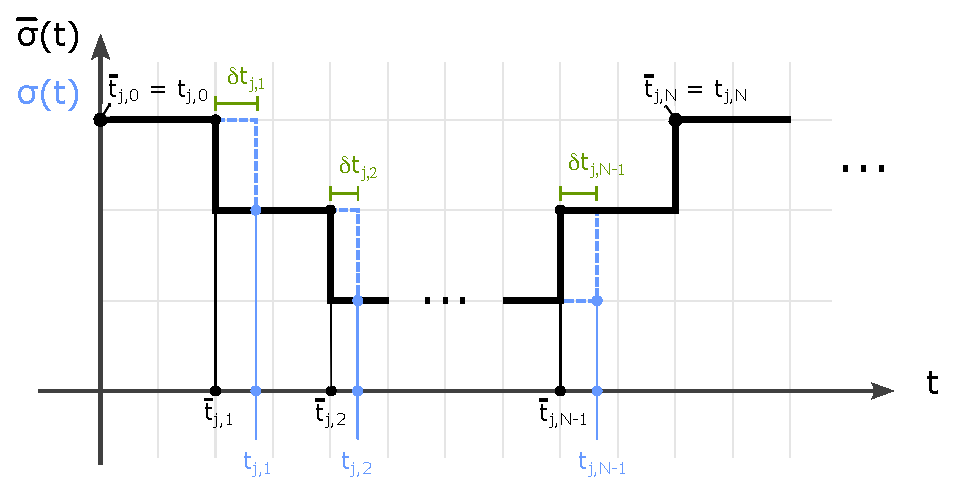
\includegraphics[]{Cap4/fig/desenho_cap4_3.eps}
%     \caption{Switching signals}\label{cap2_linearizacao}
% \end{figure}